\documentclass{standalone}
\usepackage{pgfplots}
\pgfplotsset{compat=newest}

\begin{document}
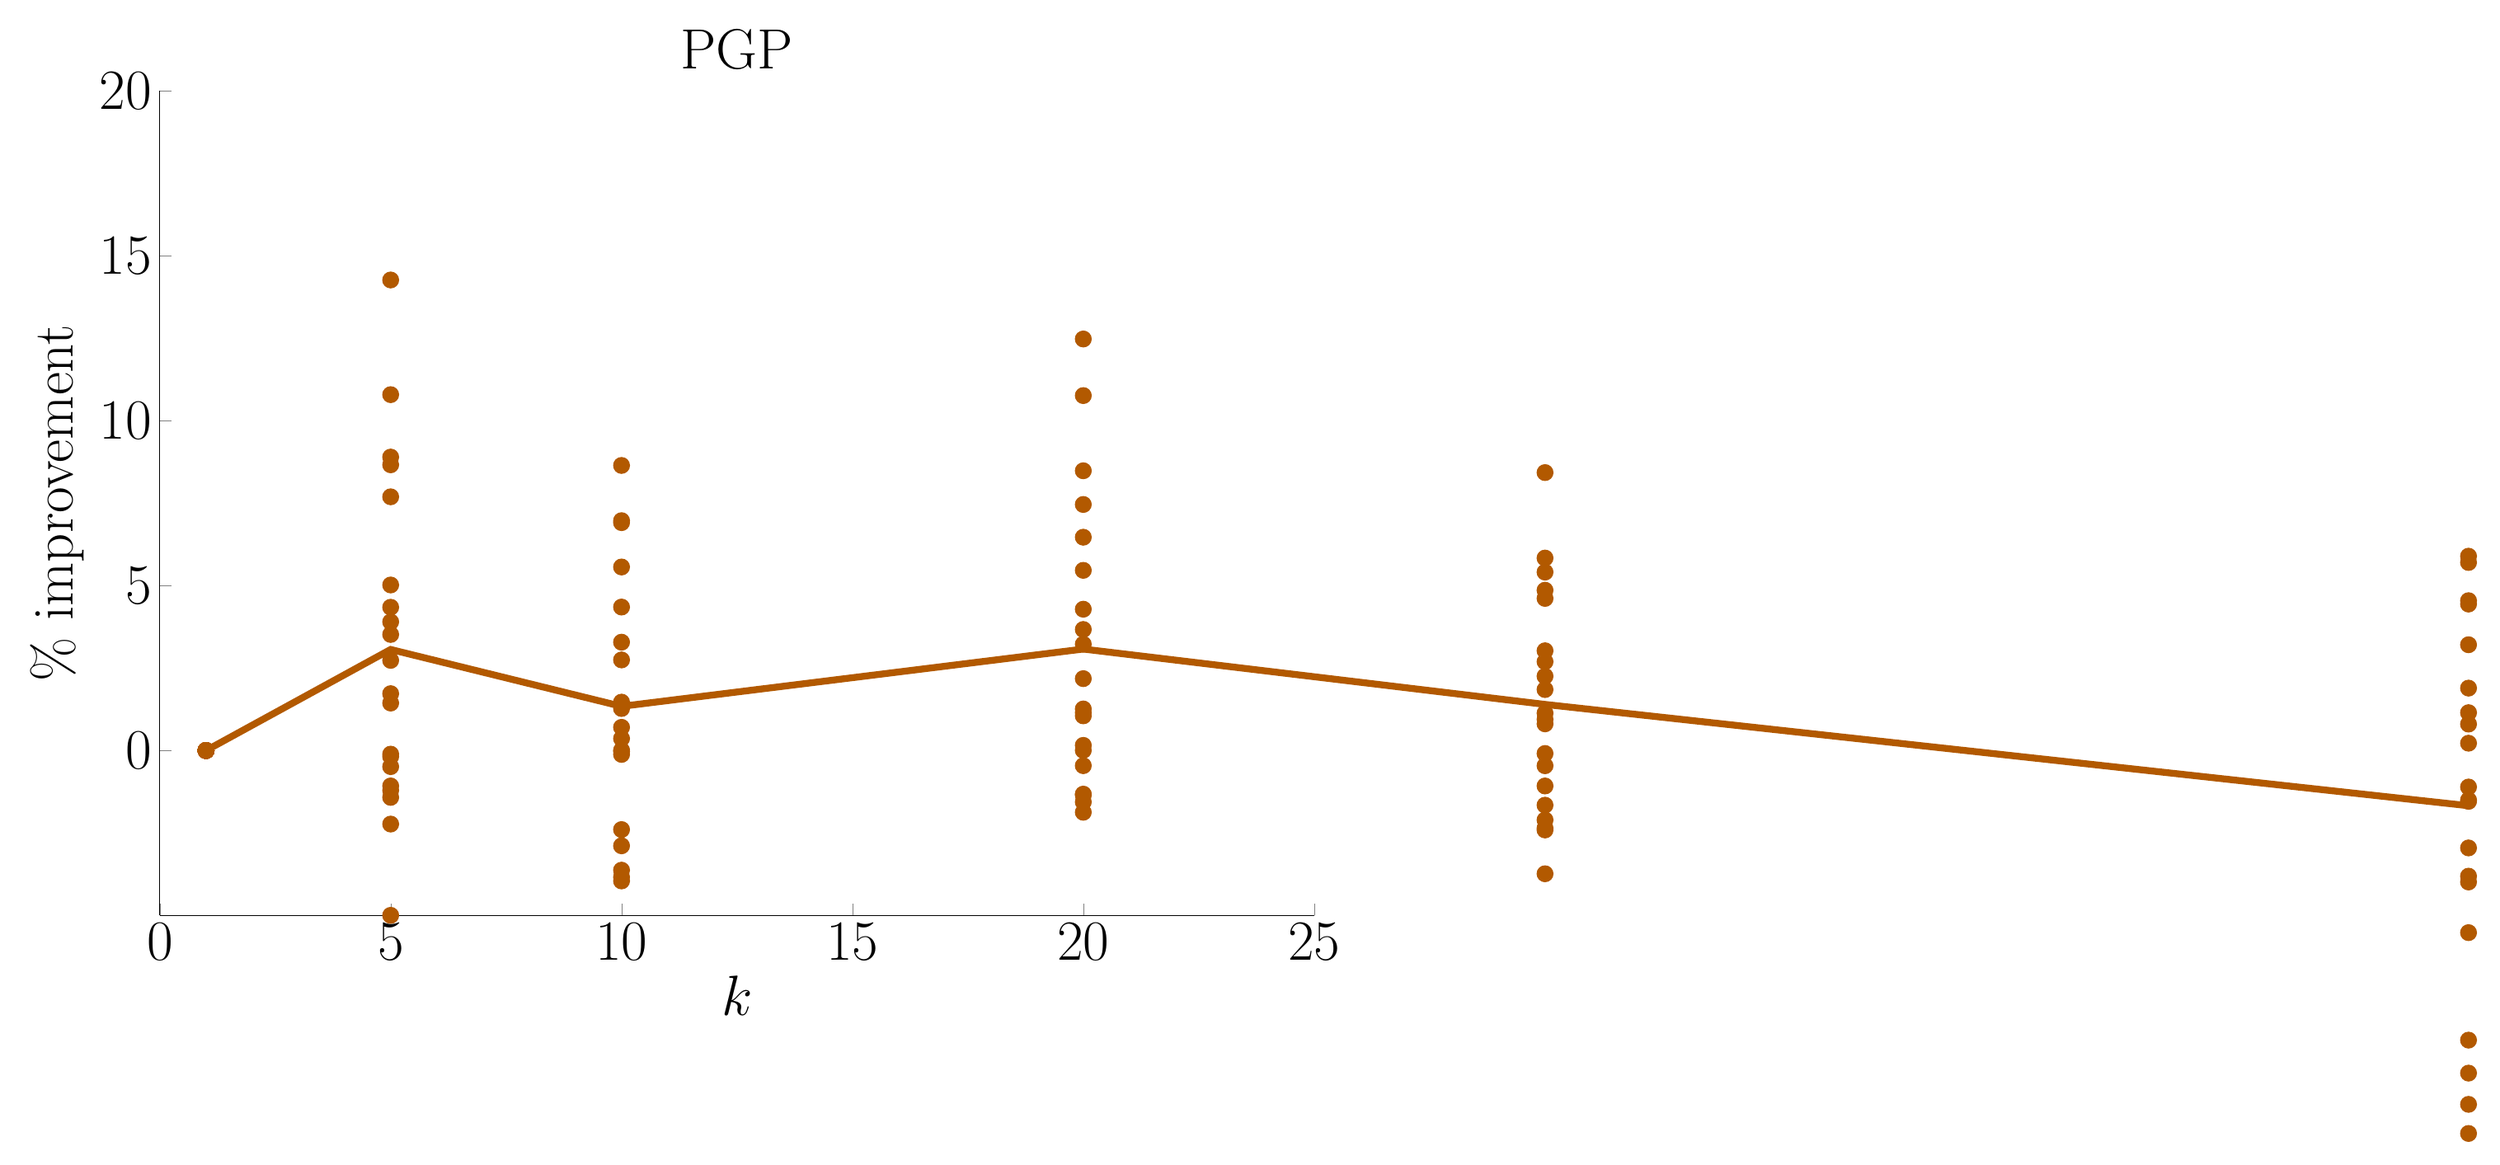
\begin{tikzpicture}

\begin{axis}[%
title style={font=\Huge},
title=PGP,
tick label style={font=\Huge},
label style={font=\Huge},
legend style={font=\Huge},
view={0}{90},
width=7in,
height=5in,
scale only axis,
xmin=0, xmax=25,
xtick={0, 5, 10, 15, 20, 25},
xlabel={$k$},
ymin=-5, ymax=20,
ytick={0, 5, 10, 15, 20},
ylabel={$\%$ improvement},
major tick length=5pt,
axis lines*=left,
legend cell align=left,
clip=false]

\addplot [
only marks,
mark=*,
mark size=3.5pt,
color=orange!70!black,
%solid,
%line width=2pt,
]
coordinates{
(1,0.0)(1,0.0)(1,0.0)(1,0.0)(1,0.0)(1,0.0)(1,0.0)(1,0.0)(1,0.0)(1,0.0)(1,0.0)(1,0.0)(1,0.0)(1,0.0)(1,0.0)(1,0.0)(1,0.0)(1,0.0)(1,0.0)(1,0.0)(5,-4.99739379724)(5,-2.22985633979)(5,-1.42027114267)(5,-1.20604475443)(5,-1.07336956522)(5,-0.4877014419)(5,-0.181561428283)(5,-0.110041265475)(5,1.43894218304)(5,1.72435336749)(5,2.73398188527)(5,3.51912568306)(5,3.90186915888)(5,4.34436318876)(5,5.01994223628)(5,7.69352540763)(5,8.6636894538)(5,8.89862516997)(5,10.7905321782)(5,14.2680310282)(10,-3.95423340961)(10,-3.83824537354)(10,-3.62712458384)(10,-2.88870008496)(10,-2.39642398907)(10,-0.117677824268)(10,-0.0293513354858)(10,0.00862477899004)(10,0.363839910439)(10,0.703857137111)(10,1.27459129953)(10,1.36208853575)(10,1.46753933087)(10,2.74743004656)(10,3.28535806466)(10,4.35091829477)(10,5.56501515844)(10,6.9102426838)(10,6.96998239076)(10,8.64440078585)(20,-1.87202700629)(20,-1.56026557712)(20,-1.34759304207)(20,-1.32162015082)(20,-0.459021643404)(20,0.00550949009669)(20,0.156600720363)(20,1.05193252756)(20,1.14789687924)(20,1.26024590164)(20,2.18032299078)(20,3.22371213824)(20,3.6706561231)(20,4.28525462895)(20,5.46344333316)(20,6.46844027126)(20,7.46059193544)(20,8.48300717839)(20,10.7628036516)(20,12.4788679482)(30,-3.73667240322)(30,-2.40859609232)(30,-2.35562941421)(30,-2.10396855028)(30,-1.65733662393)(30,-1.07435902481)(30,-0.46106557377)(30,-0.0897430284989)(30,0.809098701679)(30,0.947426299539)(30,1.13293363655)(30,1.84889761525)(30,2.25423618494)(30,2.69343894023)(30,3.02516322405)(30,4.61274574482)(30,4.86057319907)(30,5.41011131149)(30,5.83577529771)(30,8.42798316666)(50,-11.6110533447)(50,-10.7286954395)(50,-9.78106168428)(50,-8.78082988914)(50,-5.52158575508)(50,-3.98627675216)(50,-3.80997104172)(50,-2.95303091128)(50,-1.54114286636)(50,-1.50045776678)(50,-1.10632239197)(50,0.222269467906)(50,0.80179040576)(50,1.14818414138)(50,1.89267340118)(50,3.20741143649)(50,4.44063274252)(50,4.54389481859)(50,5.70194035577)(50,5.89318600368)
};

\addplot [
color=orange!70!black,
solid,
line width=3pt
]
coordinates{
(1,0.0)(5,3.06453706028)(10,1.34010659084)(20,3.07693791491)(30,1.39855063055)(50,-1.67342225349)
};

\end{axis}
\end{tikzpicture}
\end{document}
